%----------------------------------------------------------------------------------------
%	GOALS
%----------------------------------------------------------------------------------------

\section{Anforderungen, Ziele und Rahmenbedingungen}

\subsection{Empirische Untersuchung}

Zu Beginn der Anforderungsermittlung wurde eine Umfrage im Unternehmen durchgeführt, bei der die Entwickler gebeten wurden, Auskunft über die Projekte zu geben, die sie betreuen. Ziel der Untersuchung war es, mehr über die verwendeten Technologien und damit verbundenen Rahmenbedingungen zu erfahren, sowie persönliche Einschätzungen der Entwickler zu Testing und anderen automatisierbaren Aspekten der API-Entwicklung einzuholen. In diesem Abschnitt werden die Ergebnisse der Umfrage aufgeführt.\\

\subsubsection{Verwendete Technologien}

Alle befragten Entwickler gaben an, dass sie API-Projekte betreuen, die in PHP geschrieben sind. Andere Sprachen sind dabei kaum vertreten (dargestellt in Abbildung \ref{fig:sv-languages}). Als primär verwendete Frameworks wurden Symfony (60\%) und Laravel (30\%) genannt, wobei auch einige andere Frameworks zu einem geringeren Maß verwendet werden (siehe Abbildung \ref{fig:sv-frameworks}).

\begin{figure}[H]
\centering
  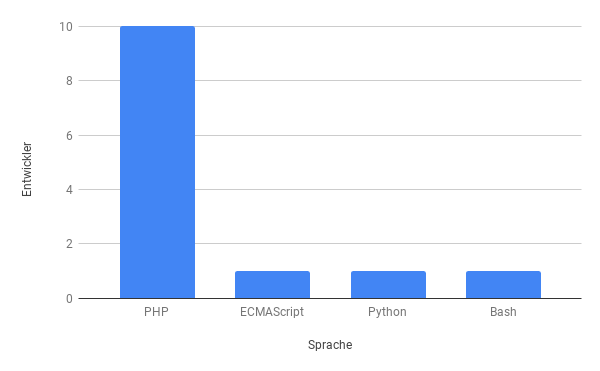
\includegraphics[width=0.8\textwidth]{../images/languages.png}
  \caption{Verwendete Sprachen}
  \label{fig:sv-languages}
\end{figure}

\begin{figure}[H]
\centering
  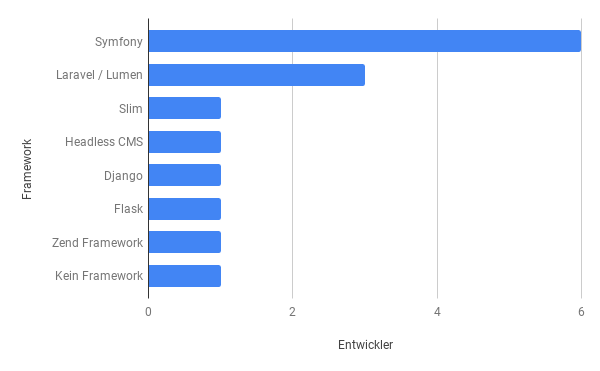
\includegraphics[width=0.8\textwidth]{../images/frameworks.png}
  \caption{Verwendete Frameworks}
  \label{fig:sv-frameworks}
\end{figure}

90\% der Entwickler gaben an, dass ihre APIs primär die REST-Architektur befolgen; die restlichen 10\% benutzen GraphQL als Grundlage. Auf die Frage, ob sie Description Languages zur Beschreibung ihrer APIs verwenden, antworteten 50\% der Entwickler positiv. Die Beschreibungen werden dabei zu 60\% manuell geschrieben, und zu 40\% automatisch aus dem Code der Anwendung generiert. Die verwendeten Description Languages sind in Abbildung \ref{fig:sv-dls} dargestellt.

\begin{figure}[H]
\centering
  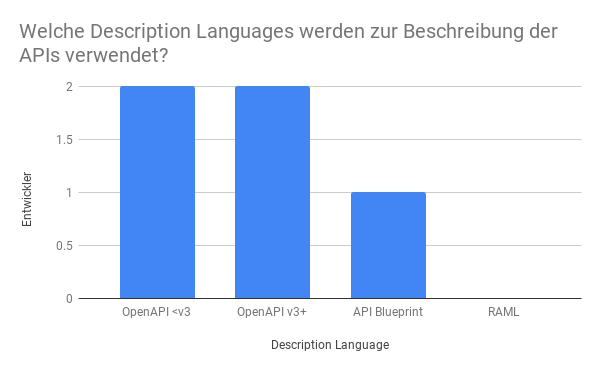
\includegraphics[width=0.8\textwidth]{../images/dl_type.png}
  \caption{Verwendete Description Languages}
  \label{fig:sv-dls}
\end{figure}

\subsubsection{Testing der APIs}

Bei der Frage wie die APIs aktuell getestet werden, fällt auf, dass viele Entwickler keine automatisierten Tests verwenden. Stattdessen werden häufig nur manuelle Tests, insbesondere mithilfe von Postman, durchgeführt. Lediglich 30\% der Entwickler gaben an, dass sie Unit bzw. Integration Tests einsetzen (siehe Abbildung \ref{fig:sv-testing}). Dennoch bewerteten die meisten Entwickler die Testabdeckung der APIs insgesamt als eher positiv, wenn auch hervorzuheben ist, dass einige APIs eine unzureichende bzw. nichtexistente Testabdeckung aufweisen (siehe Abbildungen \ref{fig:sv-coverage} und \ref{fig:sv-insufficient-coverage}).

\begin{figure}[H]
\centering
  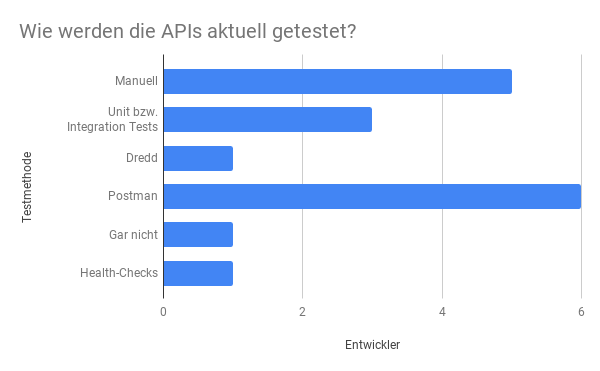
\includegraphics[width=0.8\textwidth]{../images/testing.png}
  \caption{Testing der APIs}
  \label{fig:sv-testing}
\end{figure}

\begin{figure}[H]
\centering
  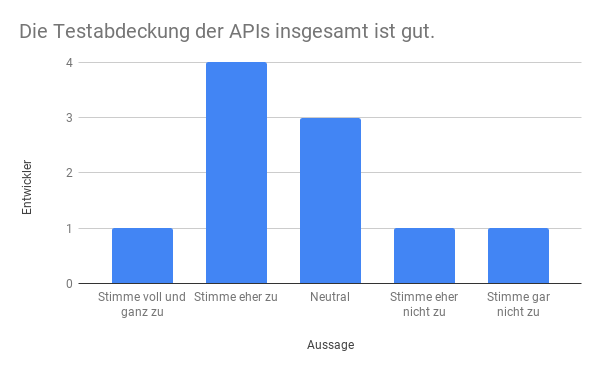
\includegraphics[width=0.8\textwidth]{../images/coverage.png}
  \caption{Testabdeckung der APIs insgesamt}
  \label{fig:sv-coverage}
\end{figure}

\begin{figure}[H]
\centering
  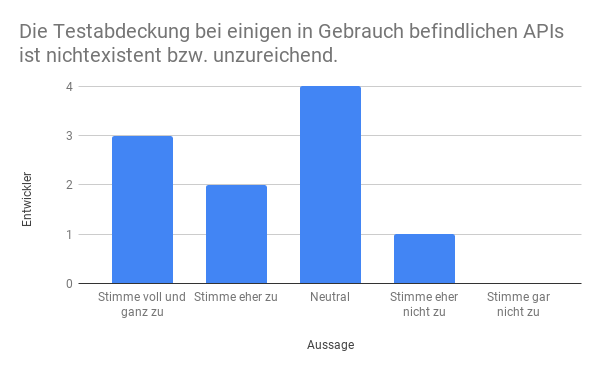
\includegraphics[width=0.8\textwidth]{../images/insufficient_coverage.png}
  \caption{Unzureichende Testabdeckung mancher APIs}
  \label{fig:sv-insufficient-coverage}
\end{figure}


\subsection{Anforderungen}

\subsection{Ziele}

Im Folgenden werden die konkreten Ziele des Systems hierarchisch angeordnet. Zunächst werden die strategischen, langfristigen Ziele festgelegt, aus denen sich anschließend die taktischen und operativen Ziele ableiten. Die Ziele sind in der jeweiligen Kategorie nach ihrer Priorität angeordnet. Bei allen Zielen wird davon ausgegangen, dass eine API Spezifikation vorliegt, auf Basis derer die Aufgaben durchgeführt werden können.

%------------------------------------------------

\subsubsection{Strategische Ziele}

\begin{enumerate}
	\item \textbf{Optimierung des REST-API Entwicklungsprozesses.} \\
	Durch zumindest teilweise Automatisierung von verschiedenen Aufgaben im Entwicklungsprozess (Testing \& Dokumentation) soll Zeit eingespart werden.
	\item \textbf{Erhöhte Softwarequalität.} \\
	Die Vereinheitlichung des Prozesses und auch die automatisierte Generierung von Artefakten sollte zu einer höheren Softwarequalität und einfacheren Wartung führen.
	\item \textbf{Vereinheitlichung des REST-API Entwicklungsprozesses.} \\
	Mit der Unterstützung des Entwicklungsprozesses durch das System sollen Grenzen und Vorgaben gesetzt werden, in denen sich die Entwickler bewegen. Das Design der REST APIs folgt einem einheitlicherem Konzept, wodurch Nutzer nicht bei jeder API mit neuen Designentscheidungen konfrontiert sind. Generierte Artefakte sind konsistent, und ihre Nutzung muss nur einmal erlernt werden.	
\end{enumerate}

%------------------------------------------------

\subsubsection{Taktische Ziele}

\begin{enumerate}
	\item \textbf{Abstraktes Datenmodell.} \\
	Das Datenmodell des Systems sollte so konzipiert sein, dass mehrere Spezifikationsformate überführt werden können.
	\item \textbf{Erweiterbarkeit des Systems.} \\
	Das System sollte so modular konzipiert und implementiert sein, dass Teile des Systems erweiterbar sind. Damit könnten beispielsweise neue Parser (zur Unterstützung von neuen Spezifikationsformaten) oder Factories (z.B. zur Generierung von Testcases in einer anderen Sprache) in das System eingebunden werden.
	\item \textbf{Generierung von Testcases.} \\
	Es sollen automatisch sinnvolle Testcases generiert werden, um die Funktionalität der API zu testen. Diese sollten dabei unterstützend wirken. Das Ziel ist es nicht, die Entwickler komplett vom Schreiben von Tests zu entbinden; vielmehr sollen einfache Tests zwar komplett automatisiert werden, bei solchen Tests, die noch manuelle Ergänzungen der Entwickler benötigen, soll das Systems allerdings nur hilfreiche Vorarbeit leisten.  
	\item \textbf{Generierung von Dokumentationsartefakten.} \\
	Zur Verbesserung der Dokumentation der API sollen automatisch kollaborationsunterstützende Artefakte generiert werden.
	\item \textbf{Überprüfung auf Best Practices.}  \\
	Es sollte (optional) auf die Befolgung von Best Practices beim Design von REST-APIs geprüft werden sollen (Linting). 
	
\end{enumerate}

%------------------------------------------------

\subsubsection{Operative Ziele}

\begin{enumerate}
	\item \textbf{Generierung von JSON Schemas.} \\
	Aus dem eingelesenen Metamodell sollen JSON Schemas generiert werden, welche unter anderem für Testcases verwendet werden.
	\item \textbf{Generierung von nominalen Testfalldefinitionen.} \\
	Zur Überprüfung der Funktionalität der API, sollen Testcases generiert werden, die jeden Endpunkt der API mit den in der Spezifikation definierten Parametern und Attributen aufrufen, und auf valide Antworten prüfen.
	\item \textbf{Generierung von fehlerhaften Testfalldefinitionen.} \\
	Es sollen nicht nur Testfälle generiert werden, die auf Funktionalität der API in Einhaltung aller in der Spezifikation definierten Einschränkungen prüfen, sondern auch solche, die auf korrekte Fehlerbehandlung prüfen. Dies kann z.B. in Form einer Anfrage mit falschen Attributen oder Attributwerten geschehen.
	\item \textbf{Generierung einer API Dokumentation}. \\
	Es soll eine responsive, interaktive und leicht anpassbare API-Dokumentation generiert werden, welche die Benutzung der API verdeutlicht.
	\item \textbf{Generierung und Synchronisation von Postman Collections.} \\
	Als weiteres kollaborationsunterstützendes Artefakt sollen automatisch Postman Collections generiert werden, und diese automatisch über die Postman API bei allen Entwicklern synchronisert werden.
	\item \textbf{Einfache Einbindung in Projekte.} \\
	Das System sollte ohne großen Aufwand in neue oder bestehende Projekte eingebunden werden können.  
	\item \textbf{Partielle Überschreibung von Testcases bei Neugenerierung. } \\
	Insbesondere bei den Testcases, die noch weitere manuelle Ergänzungen der Entwickler benötigen, sollen bei Neugenerierung nicht die Ergänzungen überschrieben werden.
\end{enumerate}

\subsection{Funktionsumfang des Prototyps}
